\normallinespacing

\chapter{State of the Art}
%Start with a title and develop your ideas from the most general to the most specific (from the topic to the specific problem). The document should conclude with your research question stated as a reasonable consequence of what you have reported and discussed.
% Context why we use machine learning model
% Why we chose triplet loss -> Avoiding predefined classes
% Use of weakly labelled data -> Quantity over quality...

In the last chapter, we saw information technology has a decisive role in shaping our society as well as some breakthroughs of the technology that altered how we manage, retrieve and distribute information and critically changed our way of thinking and living. The advancements in information technology is an ongoing central force of digital innovation in today's society. Yet we think there are a plenty of opportunities left behind. This chapter encompasses this long-running technological advances from the past, making readers certain of the state-of-the-art studies that are relevant to our work, and shows how seamlessly our methodology will progress from the current point in the next chapter. 

As seen in the introduction, information technology can mean any kind of systems for storing, retrieving, and sending information. In this work, we focus exclusively on information technology which deal with information that are processed and structured from audio data. 
More specifically, with our proposed methodology, we contribute to the research of content-based audio retrieval which allows people to access sounds efficiently and intuitively by looking inside a cluster of sounds grouped by content-based similarity instead of examining a linear list of audio content.
To achieve this, we think of two independent issues which are equally important: the way of representing sounds (production of audio features) and the way of presenting sounds based on the given representation (clustering approach). We discuss these two issues in the context of an information retrieval process.% which begins when a user enters a query for sounds into the system and finds matching objects. There is no doubt that such a system greatly helps people's search for digital sounds on the internet which is increasingly daunting because of the information overload we discussed in the last chapter.


The following sections offer a collection of the most up-to-date work and ideas regarding audio retrieval.
%We give a special importance to the context of why an effort of research or development was made and what problem did it try to address. In this way, we might have to give up some trivial facts and details of the topic, but we believe it is inevitable so that readers can focus on a contiguous progression of previous development toward our proposed method in the next chapter. 
Each of the following sections is dedicated to a fundamental technique of our methodology. 
The rest of this chapter is organized as follows: in the next section, we discuss the most general topic of our research: information retrieval, focusing on its connection to sound and music computing instead of going into detail of applications with non-audio information. Then, in Section 2, a class of traditional audio features, the building blocks of audio retrieval, are introduced. In Section 3, we cover the audio features that are recently developed with the help of deep learning. Then, among those new kind of features, we focus on those learned from similarity learning and discuss its practical use for sound retrieval in Section 4. In Section 5, a review of clustering methods is presented with the focus on two popular approaches, the partitional clustering and the graph-based clustering. Due to the large volume and many topics to be covered, Figure~\ref{toc-figrue} visualizes the thematic structure of the following sections and allows readers to focus on specific topics.

\begin{figure}[htb]
	\centering
	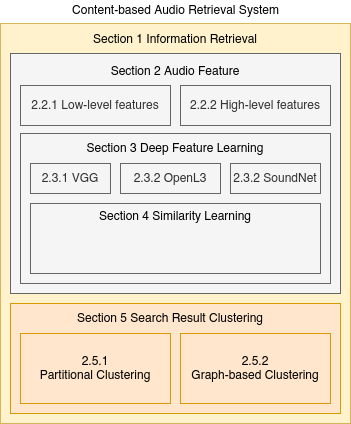
\includegraphics[width=7cm]{Figures/conceptual_relationship_of_sections.png}
	\caption{Overview of the sections in this chapter. Each section in the same group shares a topic in common.}
	\label{toc-figrue}
\end{figure}

\section{Information Retrieval and Audio}
The purpose of this section is to emphasize that our work lies at an intersection of information retrieval (IR) and audio engineering problems, pointing out a close relationship between IR systems and audio engineering with examples. We introduce fundamental technologies that are essential to modern IR process such as database technology. Also a number of terminologies used in the IR research, which appear thoroughly in the following sections, are carefully introduced since those may not be clear for readers from audio engineering backgrounds.

\subsection{Information Retrieval}

Information retrieval is the science of finding information that satisfies an information need from a large collection of those resources~\cite{manning2008}. Most IR systems start off by taking as input a text, a search query which describes user's information needs formally or informally, for example search keywords for web search engines. Then, given a query, the system ranks the data objects which are represented by information in the database. The rank of relevance between the query and each object is measured using a numeric score on how well the object matches with the query~\cite{guandong2010}. Then, it shows the top ranking objects to the user. While traditionally IR is used to mean searching for documents (an unstructured text data) from a collection of other documents in computers~\cite{manning2008}, IR is becoming the dominant form of any kind of information access. Today, the objects that IR systems deal with are not only texts but a wide variety of multimedia data are also supported such as images~\cite{abby2000} and sound~\cite{jonathan1999}, and the retrieval process can be performed using either full-text query or content-based query~\cite{lew2006}.

Techniques and algorithms which enable efficient retrieval process vary with the kind of information to search for. For example, Music Information Retrieval (MIR), which is a branch of IR and deeply related to our work, focuses on retrieving information from music. Since our work focuses on the research and development of content-based audio retrieval which aim to deal with a various types of sounds, including artificially-created sounds such as music loops, we will come back to this topic (see Section~\ref{sec:mir}) and discuss advances in techniques and knowledge of the MIR research. 

\subsection{Database System}
As already mentioned, database system is one of the underlying technologies in IR.  It is employed in any kind of web-based applications~\cite{williams2004} and makes possible an satisfying IR experience on the internet . However, database searching itself is not considered as IR because it lacks the ranking process of the search results~\cite{jansen2010}. This means an IR system returns the results which may or may not match the query in the order of relevance while typically a database system returns nothing when no matching object is available in its data collection. Furthermore, an IR system does not limit the user to a specific query language while such languages like SQL or MongoDB are commonly used in database systems~\cite{karan2017}.
Despite the key differences, it is worth taking a close look at the database technology, specifically in regard to web services, because it is an integral part of many popular web-based IR systems, for example image retrieval on Flickr and audio retrieval on Freesound, and importantly, some of those applications will appear as examples in the following sections. 

\subsubsection{Database on the web}\label{DBonWeb}
Considering different concerns, a website is usually separated into two independent components: one that considers the activity of clients, helping them interact with data on a website, and the other that takes command of the web servers which essentially provide service to one or many clients. Many users of the internet, even non-technical users, know fairly well about the first part, especially the graphical user interfaces (GUI). The development of such interfaces is known as front-end web development. The interfaces are designed using programming languages such as HTML, CSS, and JavaScript, that can be executed on client devices with a web browser. Modern front-end development is accustomed to support intuitive GUIs and often built on the top of commonly-shared templates, among which the most popular one is Twitter's Bootstrap\footnote{https://getbootstrap.com/}. As such, most of users who already got used to modern web experience will easily guide themselves when they visit a new website.

What's often left invisible and unknown to the public is a large number of server-side processes running in the back end. Through front end interfaces, users can communicate with the server of a website and properly command them to return the data they look for. Efficiency of the back end system highly affects the performance of the front end activity. Indeed, even basic user experience such as authentication and permission, requires communicating and retrieving data stored in server-side database systems. As such, the database for the website is placed and accessed in the back end.

\subsubsection{Database in practice}
A database system and a file system have some functions in common and the similarity of two systems may confuse some readers. Practically, both system store the data in files: a database system stores data with predefined data formats in a table and a file system stores data (the pointers which indicate where and what data is stored in a hardware storage).

% Maybe About SQL and NoSQL for querying

% Maybe About RAID6 for secure database

% Maybe About how data is typically organized, not nested much



\subsection{Multimedia Information Retrieval}
\label{sec:mir}

\subsection{Freesound}
Freesound\footnote{https://freesound.org/} is a non-profit organization which hosts a collaborative web-based repository of Creative Commons Licensed sounds. It has been maintained at the Music Technology Group (MTG) in Universitat Pompeu Fabra, Barcelona. The repository was launched in 2005 with an initial goal to provide a large royalty-free sound databases with sound researchers to test their algorithms~\cite{frederic2013}. Since then, it has widely adopted by sound artists, application developers and all sorts of content creators and became a standard website for sharing Creative Commons sounds.

%Way of Browsing -> Information Retrieval
%Analysis -> Audio features, Essential

\begin{figure}[htb]
	\centering
	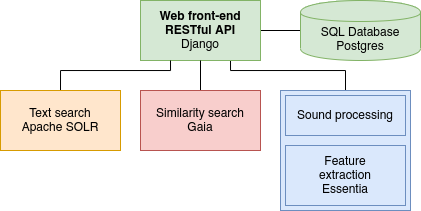
\includegraphics[width=10cm]{Figures/freesound_api.png}
	\caption{Overview of system architecture of Freesound~\cite{frederic2013}. The architecture is a good example of the use of database system in web-based IR systems as discussed in the Section~\ref{DBonWeb}}
	\label{freesound-api}
\end{figure}


% \subsection{Content-based and context-based search \texttt{<in progress>}}
% % Context ... user-generated tags and descriptions
% % Content ... Audio data itself
% % What are the SoTA application examples from two approaches

% Two underpinnings for audio retrieval are how audio data is represented (audio feature) and how data will presented to users. Before breaking down the two topics in the following sections, this section aims to provide readers with a context for the sound retrieval research, covering from historical examples to an example of popular real-world application, explaining emerging technological advancements which affect its future research directions.

\subsection{Toward intelligent audio retrieval}
So far, we have seen various efforts made in the research and development of efficient IR for multimedia information, focusing on audio. Speaking of audio retrieval, humans are inherently good at remembering/retrieving audio since we are born with a set of abilities to discriminate a wide range of sounds, especially in the context of speech. Moreover, we are also able to relate and match similar sounds~\cite{denise1995}. In fact, we have the capability to detect and relate sound events or “acoustic objects” which we have never encountered before, based on how that phenomenon stands out against the background~\cite{kumar2014}. To computers, however, a raw audio signal data is essentially a featureless collection of bytes with most rudimentary information embedded such as file name, format, and sampling rate. This does not readily allow efficient management and searches for sounds. To accomplish the task, we first need to transform sounds into a small set of parameters (audio features) and, in the next section, we will go into detail of various analysis techniques to achieve this goal. 

\section{Audio Features} 
In machine learning and pattern recognition, a feature is most briefly defined as an individual measurable property or characteristic of a phenomenon being observed~\cite{bishop2006}. Features that appear in this work are always real-valued numeric while they may vary in different contexts such as binary (e.g. "on" or "off"); categorical (e.g. "A", "B", "AB" or "O", for blood type); ordinal (e.g. "large", "medium" or "small").

Feature extraction is also an active research topic in multimedia IR. In case of image retrieval system, IR systems traditionally relied on manually created textual annotation to measure the relevance between user's query and information in resources (keyword annotation paradigm)~\cite{yong1998}. With the rise of the amount of information, however, the annotation approach had to be replaced with a faster and automatic feature extraction. Researchers found that the use of low-level visual features such as shapes and colors can be superior to traditional annotation-based approach in terms of robustness because automation removed the human subjectivity~\cite{jalal2016}.
 Furthermore, features are used to map from a large, complex data space into a small, simple feature space so that the system looks for information in a smaller search space efficiently~\cite{dragos2000}. 

 In regard to audio retrieval, audio features lie at the heart of our work.  Within a scheme of typical audio retrieval applications, audio features are obtained in a preliminary process, which is referred as a feature extraction process, since the raw signal is too large, noisy and redundant for most of the interesting analysis~\cite{bello2016}. In this context, feature extraction is a process that convert the raw audio waveform (time series data points) into a set of numerical vectors.  

This section aims to offer a review about two general classes of audio features, acoustic features and symbolic features, that researchers and developers commonly find useful for a range of audio applications. Audio features discussed in this section are crafted in traditional approaches and based on from low-level features such as fundamental frequency and harmonicity of signals to high-level features which are designed to provide semanticity of sounds such as "sharpness". 

\begin{figure}[htb]
	\centering
	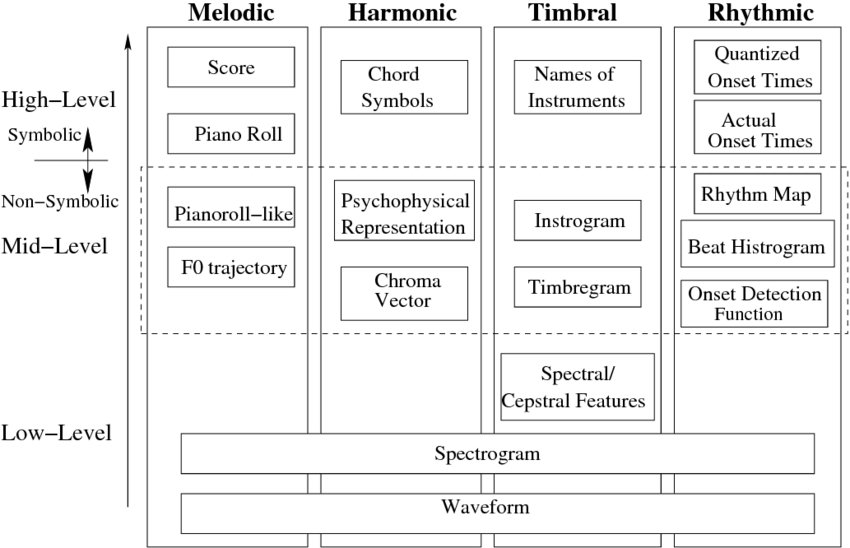
\includegraphics[width=10cm]{Figures/low-to-high-features.png}
	\caption{Classification of features into low-level, mid-level and high-level
features as suggested in \cite{ramaseshan2013}. Low-level features are obtained from the audio content, while high-level features are symbolic representation of music.}
	\label{low-to-high}
\end{figure}

\subsection{Acoustic features}
Pitch, loudness, and timbre are the acoustic features which are traditionally used to describe sounds and commonly used in many audio retrieval applications~\cite{erling1996, tzanetakis2002, kumar2013}. Those features are closely related to our audio perception and sensory stimuli we receive when we hear sounds. Audio perception is itself a complicated discipline. Interested readers are referred to~\cite{moore2003, bregman1990} to find a complete coverage of audio features and their effects on perception. Normally, acoustic feature extraction is applied to a short frame of the original signal, computing features roughly once every 10 ms over a window of 20 or 30 ms. It is important to note that this windowing operation, assuming the acoustic feature between a frame is constant, lose information from the original signal. The information loss is often perceptually trivial as long as the parameters are properly tuned for the specific application.

\subsubsection{Pitch}
% Copy-pasting
\textit{Pitch} is a perceptual frequency-related scale estimated by taking a series of short-time Fourier spectra. For each of these frames, the frequencies and amplitudes of the peaks are measured and an approximate greatest common divisor algorithm is used to calculate an estimate of the pitch. A perfect young human ear can hear frequencies in the 20-Hz to 20-kHz range and most of the application are configured to identify pitch within this range as accurately as possible.

\subsubsection{Loudness}
%That attribute of auditory sensation in terms of which sounds can be ordered on a scale extending from quiet to loud
Loudness is an acoustic feature with which sounds can be ordered on a scale extending from quiet to loud, describing the subjective perception of sound pressure~\cite{sonn1073}.  It is approximated by the signal's root-mean-square (RMS) level in decibels, which is calculated by taking a series of windowed frames of the sound and computing the square root of the sum of the squares of the windowed sample values.

\subsubsection{Timbre}
% Timbre is everything not Pitch and Loudness
% More complicated than Pitch (Hz) and Loudness (db)
%\subsubsection{Brightness \texttt{<in progress>}}
%\subsubsection{Bandwidth \texttt{<in progress>}}

\subsection{Symbolic features}
Unlike acoustic features which are commonly used to many different purposes, symbolic audio features are designed for a specific purpose and deeply reflected by application specifics. Figure~\ref{low-to-high} shows a class of popular audio features used in n Music Information Retrieval research, including both acoustic and symbolic features. Take an example of the high-level features, \textit{Score} and \textit{Piano Roll} are essential in applications such as melody analysis but not always required for other applications such as beat detection. This is why those are classified as high-level features from the \textit{Melodic} category.

\subsection{Feature Extraction in Practice}
In the context of the typical audio engineering development, it is usual that a developer uses freely available software for feature extraction tasks instead of coding them from scratch. This is because feature extraction processes demand a very careful optimization to the extent that only those who have considerable expertise in can achieve and, more importantly, there are a number of reputable open-source libraries in this venue~\cite{mcfee2015, giannakopoulos2015, bullock2007}. Among them, Essentia~\cite{bogdanov2013} is an open-source audio analysis tool which powers the similarity search functionality of Freesound. This library supports an extensive collection of reusable algorithms for audio feature extractions as shown in the complete list\footnote{https://essentia.upf.edu/algorithms\_reference.html}. 

As for low-level acoustic features, Essentia supports a multitude of features such as loudness, dynamic range, zero crossing rates, as well as many spectral-based features including MFCCs, spectral energy, and pitch salience. Furthermore, many other algorithms are distinctly categorized for specific applications, such as mood detection, key detection, melody extraction and audio fingerprinting, and each algorithm is regarded as a high-level feature extractor.

\section{Deep Feature Learning}
% How NN works for dimentionality reduction. It should be discussed already in the previous section that dimentionality reduction is one of the most important aspects in (traditional) feature extraction.

As introduced in the last section, traditional approaches which more or less require audio-specific domain knowledge were dominant in this field. However, recently, the use of deep learning has seen growing popularity and success. The new approach replaces laborious feature engineering in the past with automated feature learning powered by the use of neural networks. The application of deep learning techniques for the purpose of feature extraction is known as deep feature learning or deep representation learning. In this section, we go into detail of recent advancements in machine learning research in the context of audio feature learning.

\subsection{Neural Network}

Neural networks are computing systems vaguely inspired by the biological neural networks that constitute animal brains [1, Wikipedia]. Neural network is known to be able to powerfully model a highly non-linear relationship between its input and output. The training of such models can be mainly divided into two phases: training and backpropagation. Here, we refer to supervised learning approach as an example of the training of neural networks. To understand the variation of the approaches to train neural networks, readers are recommended to refer to [[this]]

As similar to the electric signals passing through each connection (synapses) and edges (neurons) in animal brains, each edges in neural networks receives a real number (signal) and apply non-linear process to it, then signal to other connected edges. At the end of the network, the neural model make outputs (often a prediction). The error of the training is computed by comparing the outputs with the target outputs. 

After computing the error for an input, the network propagates the error to the entire network from back to the front. This propagation of the error from the output layer to the input layer is known as backpropagation. During backpropagation, the network then adjusts its weighted connections according to a learning rule, such as learning rate that defines the scale of the error at given adjustments. Successive adjustments will cause the neural network to produce output which is increasingly similar to the target output. After a sufficient number of these adjustments the training can be terminated based upon certain criteria.

\subsection{Convolutional Network}
From the most simplest network such as feed-forward network to the recurrent neural network such as LSTM, there are many variations of neural networks in terms of its topological differences [Topology of a Neural Network, Splingerfield].

Regarding to deep feature learning for audio applications, convolutional neural network (CNN) is one of the most standard architecture. CNN is initially developed for computer vision tasks but

\subsection{Strategy of Deep Feature Learning}
There are three common strategies that facilitates the learning of sound representations. Different strategies are suitable for different experimental settings, e.g., the size of the dataset available. In the following sections, we first describe the classic classification-based strategy that relies on classification tasks and uses the trained classifier as an extractor of sound representations. Then, it is followed by the self-supervised learning strategy that employs contextual constraints between audio and another modal, such as audio-visual correspondence in a video. Finally, we introduce the similarity learning strategy, which is the choice of our work, that optimizes sound representations directly in its feature space.

\subsection{Classification-based Strategy}

\subsection{VGG}
VGG is a Convolutional Neural Network architecture proposed by Karen Simonyan and Andrew Zisserman of Oxford Robotics Institute in 2014~\cite{simonyan2015}. It was submitted to Large Scale Visual Recognition Challenge 2014 (ILSVRC2014) and the model achieves 92.7\% top-5 test accuracy in ImageNet.
Originally, the VGG model takes an RGB image as input and passe the image through a stack of convolutional layers, where the filters are used with a very small receptive field: 3x3 (which is the smallest size to capture the notion of left/right, up/down, and center). At each layer, the results are followed by non-linear activation and max-pool. Max-pooling is performed over a 2x2 pixel window, with stride 2. The objective of max-pooling is to down-sample an image representation, reducing its dimension and allowing for generalization of the input representation in a lower dimension.
With its relative simplicity of implementation and superior performance, it has became one of the standard baseline models in the computer vision research.

The architecture of VGG model is specifically optimized for image classification tasks, however, the architecture has also gained popularity in the audio research field. Since spectrogram can be essentially treated as if a 2 dimensional vector like a grayscale image, a simple adaptation to an audio task is possible relatively easily by changing the input layer to a spectrogram input.

\subsection{Case: AudioSet}
Sound representations  from AudioSet \cite{jort2017} use a spectrogram-based CNN architecture trained on a classification task.

\subsection{Case: OpenL3}
OpenL3~\cite{cramer2019} also uses a spectrogram-based CNN architecture but trained through self-supervised learning of audio-visual correspondence in videos.

\subsection{Case: SoundNet}
About SoundNet and how it extracts features

\section{Similarity Learning}
%Classification in machine learning is a supervised learning in which the computer program identifies to which of a set of categories a new observed data belongs, on the basis of a training set of examples consisting of pairs of instances and its category. Classification models have many applications and a variety of the trained models is already used in our everyday life, such as in image recognition\cite{szegedy2015, andrew2017}, speech recognition~\cite{yanzhang2018}, and e-mail spam filter~\cite{emmanuel2019}.
In the previous section, we have seen four audio classification models and the use of those models for the production of audio features. Generally, these audio features are obtained as by-products of independent classification tasks such as environmental sound classification. While the approach has seen growing popularity and success, it comes with several drawbacks if it aims to make more expressive audio features.

First, classification learning enables a classifier to identify an observed data with a probability distribution over a set of categories (probabilistic classification), but the task is performed without a measure of similarity. It explains how probable the new input belongs to a category but ignores how similar it is to other data from the existing category. This missing particulars are crucial to feature representations. This is because, with the learned feature representations, our goal in this work is to make use of it for better organization of information represented by audio features, grouping them in a way that looks coherent to human, dealing with data that are not observed in the training set of data.

Similarity learning is also an area of supervised machine learning, which is closely related classification approach~\cite{andrew2018}, but it considers similarity. The goal is to learn to estimate how similar a feature is to other features by optimizing a similarity function that measures a distance in the feature space. However, in spite of being specialized in similarity, a large body of work has focused solely on features trained with classification-based approaches and similarity learning did not enjoy much attention. For example, the idea of using neural networks to extract features that respect certain relationships dates back to the 90s. Siamese Networks~\cite{bromley1993} find an feature space such that similar examples have similar features and vice versa. However, it was not feasible to train such a neural network given the limited compute power at the time~\cite{chao2017}.

With sufficient data, computational power, recent advancement in machine learning allowed for the training of Siamese architecture. Sampling strategy, appropriate distance metric, and the structure of the network are the challenging factors for researchers to improve the performance of the network.  In this section, we introduce several principles and methods regarding similarity learning, giving special importance to the details of the architecture based on triplet loss.

\subsection{Learning Approach}
\subsubsection*{Supervised Learning}
\subsubsection*{Weakly Supervised Learning}

\begin{figure}[htb]
	\centering
	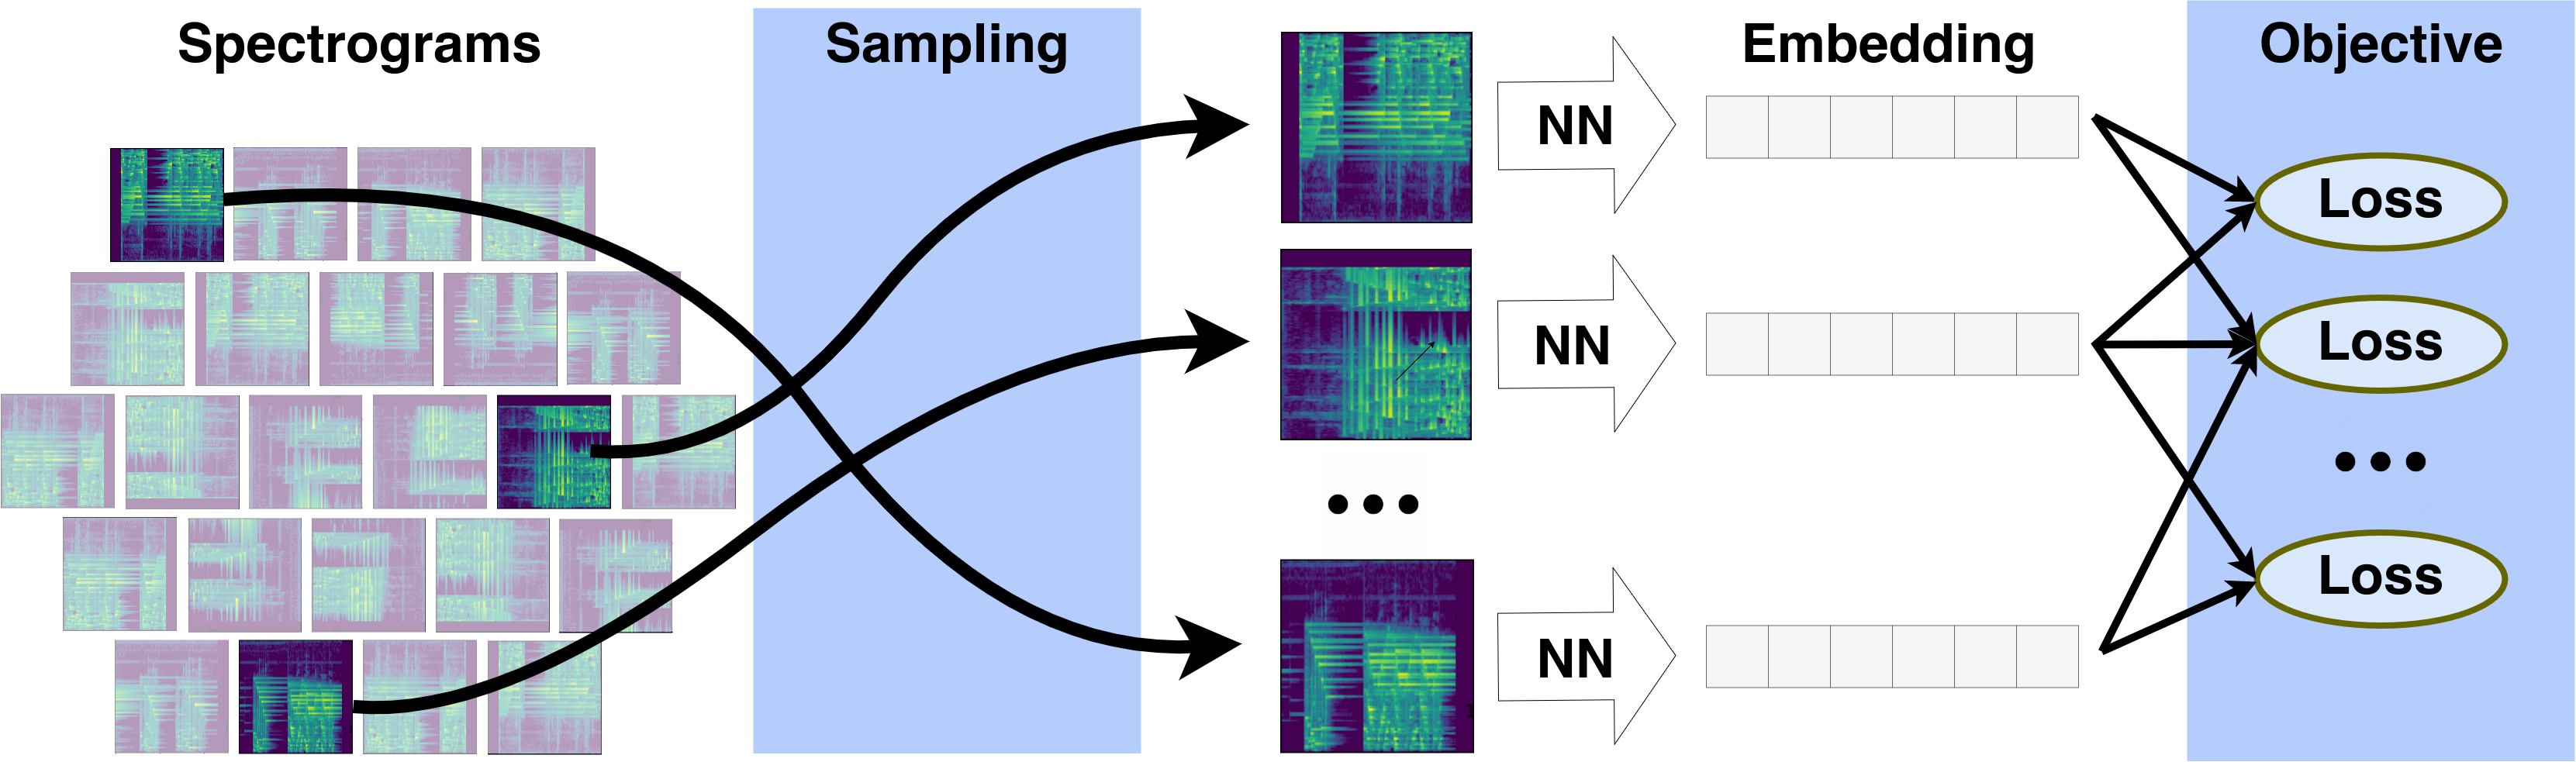
\includegraphics[width=13cm]{Figures/learning_scheme.png}
	\caption{\texttt{\textbf{Similar architecture for audio application will be shown}}}
	\label{deep-model}
\end{figure}

\subsection{Triplet Mining}
It is known that choosing (mining) which triplets to use are essential for achieving good generalization in similarity learning~\cite{schroff2015}. The importance of triplet mining is intuitively and concisely given in~\cite{hermans2017} while focusing on person re-identification tasks. Borrowing the idea and putting it in the context of audio retrieval, it can be described as follows: telling over and over again that sounds with different acoustic properties are different sounds does not teach the model anything, whereas listening to similarly-sounding but different sounds (hard negatives), or wildly different sounds of the same category (hard positives) dramatically helps understanding the concept of “sound category”. 

%MOVE
The idea to use hardest examples is critical but it may lead to local minima early in the training~\cite{schroff2015}. To address this concern, a workaround is commonly applied, which is considered as "moderate" since it finds the hardest examples from a small batch instead of the hardest one in the dataset~\cite{hermans2017, yesiler2020}.

Also, when triplet loss is used with a large amount of data, the number of possible combination of triplets easily explodes. To solve these problems, we need to formulate triplet mining strategy which ensures the difficulty of triplets 

\section{Clustering}
From an application perspective, our work strives for shift from the traditional audio retrieval to a more knowledgeable approach which provides users with content-based relationships between sounds to access what they look for. The new intelligent way of audio retrieval is analogous to the process of knowledge acquisition. 
Essentially, knowledge acquisition is the process of storing new information in memory in a way that it can be efficiently retrieved later~\cite{danielle2002}. The efficiency of this process depends largely on the representation quality of the information and also how they are organized in the storage. Take for instance, language acquisition is not only about memorizing a large vocabulary but what's also important is the organization of such information, grouping vocabulary by semantic similarity (synonyms) or putting them in a context with sentences.

So far, we have seen the recent advancements in the studies that aim to convert featureless audio signal into a expressive but compact representation of the acoustic information. We concluded in the last section that audio features learned with similarity learning are the most suitable for our purposes. In this section, we discuss the later part, clustering: the task of organizing a set of objects in such a way that objects in the same group (called a cluster) are more similar (in some sense) to each other than to those in other groups (clusters).

In our work, we are interested in audio features which are the informational representation of audio data and constructed exclusively on a basis of similarity among sound samples. Therefore, it is reasonable to organize such information in a way that puts similar objects closer and distant ones more distant. In this way, the presented group of audio features resembles knowledge in aforementioned knowledge acquisition process. Mathematically speaking, such algorithm belongs to a class of the cluster analysis which requires a distance function so that it measures the distance between objects (audio features).

In this section, we introduce k-Means clustering and adjusted rand index which is the procedure and measure we used to evaluate the clustering performance based on our learned features. Before moving to a specific method, we review the use of clustering algorithms in the context of information retrieval. Specifically, we discuss search result clustering which is an integral part of our research and provide an several review of previous applications in the field.

\subsection{Search Result Clustering}
Search Result Clustering (SRC) is a challenging algorithmic task that requires partitioning the results returned by search engine into classes. This process of partitioning is called Clustering. More specifically, it is a process of organizing similar search results into the same cluster so that each result belongs to a coherent and thematic cluster. Usually, when a traditional search engine is given an ambiguous query, the search engine tries to satisfy this query with high recall, meaning it returns many results which are not necessarily relevant to the user's information need~\cite{ugo2012}. SRC assists users in such a situation, allowing them to look through the clusters of relevant topics without refomulating the query.

Yippy\footnote{https://yippy.com/} is a sophisticated example of search engine with an extensive SRC support which receives over 400,000 visitors a month (based on the analysis by SimilarWeb\footnote{https://www.similarweb.com/website/yippy.com}). Yippy itself does not parses and indexes the webpages on the Internet as an usual search engine does. Instead, it works as what's called meta search engine~\cite{glover2000}, giving users efficient ways of examining a large volume of search results that it obtains from multiple search engines. With the search query \textit{barcelona}, for example, the SRC process on Yippy resulted in 632 clusters from a large clusters labeled \textit{Hotel} and \textit{Lionel Messi} to smaller ones such as \textit{Airport}.

% How long do typically users spend on Freesound to check if a sound is good?
SRC is also a commonly-researched topic in the context of online sound collections where a wide variety of sounds are freely shared, such as the aforementioned Freesound. Searches for audio sounds are particularly time-consuming because users cannot skim across the results as they do in text searches and have to spend at least a few seconds to listen to the sound. Furthermore, in these platforms, the collection is generated by its users instead of coming from professional studios. This results in non-uniformly annotated content compared to professional libraries, which involve experts for annotating and organizing the collections~\cite{frederic2013}, and finding a desired sound in online sound collection by a search query is more difficult and less consistent~\cite{xavier2020}.
Therefore, the technique to identify useful subsets in their results is immensely valuable for the search in sound collections. 

Many approaches to obtain audio features were already introduced in the last section. In relation to SRC, audio features which requires a large taxonomy such as AudioSet~\cite{jort2017} is not suitable. This is because a large size of taxonomies is not applicable in the context of everyday sounds and online collections where the content to describe is too diverse and involves many different types of concepts. This increases the cost of labeling and also introduces technical difficulties such as unbalanced dataset and inability to cluster sounds properly which are unknown in the existing taxonomies. On the other hand, since similarity learning does not require a predefined classes and train audio features directly using a distance metric, sounds which belong to none of existing clusters will ideally be put aside distantly from other clusters.

 The interesting research topic is how the difference in audio features influence the performance of the clustering tasks. This is because clustering approaches we will discuss in the following sections, makes full use of given audio features for clustering unlike a classification task in which a model learns to get rid of irrelevant information from given representations. This also indicates the quality of the representation is crucial to the performance of the clustering process. %Specifically, we focus on Search Result Clustering \cite{Carpineto2013} in the context of online audio collections which use sound representations to organize search-result audio content into coherent groups in the context.
 
 
\subsection{k-Means Clustering}
Partitional clustering is a class of clustering methods that require the number of clusters to be defined before starting the process. K-means clustering is the most popular implementation of the partitional approach and it aims to partition $n$ observations into $k$ clusters in which each observation belongs to the cluster with the nearest means (cluster centers or cluster centroid).

\begin{figure}[htb]
	\centering
	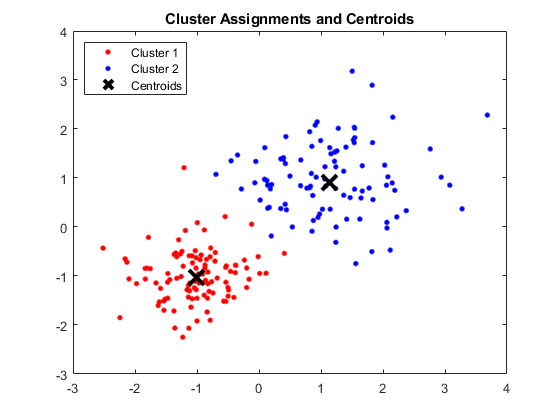
\includegraphics[width=10cm]{Figures/kmeans_diagram.png}
	\caption{}
	\label{kmeans-diagram}
\end{figure}

\subsection{Adjusted Rand Index}



\newpage


